\documentclass[12pt]{article}
\usepackage{graphicx} % Allows including images
\graphicspath{{../figures/}}
\usepackage{booktabs} % Allows the use of \toprule, \midrule and \bottomrule in tables
\usepackage{amsmath, amssymb, amsthm, gensymb}
\usepackage{mathtools}
\usepackage{hyperref}
\usepackage{epigraph}
\usepackage{etoolbox}
\usepackage{listings}
\usepackage{exercise}
\usepackage{multirow}
\usepackage{array}
\newcolumntype{C}{@{}c@{}}
\newcommand{\bottombox}[1]{\makebox[2em][r]{#1}\hspace*{\tabcolsep}\hspace*{2em}}%
\newcommand{\innerbox}[2]{%
    \begin{tabular}[b]{c|c}
       \rule{2em}{0pt}\rule[-2ex]{0pt}{5ex} & \makebox[2em]{#2} \\\cline{2-2}
       \multicolumn{2}{r}{{#1}\hspace*{1.5\tabcolsep}\hspace*{2em}\rule[-2ex]{0pt}{5ex}}
    \end{tabular}}
\renewcommand{\arraystretch}{1.25}
\makeatletter
\patchcmd{\epigraph}{\@epitext{#1}}{\itshape\@epitext{#1}}{}{}

\usepackage{tikz}
\usetikzlibrary{shapes,arrows,positioning}
\usetikzlibrary{arrows.meta}
\usetikzlibrary{chains,fit,shapes,calc}
\usepackage{adjustbox}
\usepackage{physics}

\newcommand{\uvec}[1]{\textbf{#1}}

\newtheorem{exe}{Exercise}
\newtheorem{program}{Programming exercise}
\newtheorem{theorem}{Theorem}

\usepackage{exercise}

\DeclareMathOperator{\Hessian}{Hess}

\definecolor{myblue}{RGB}{80,80,160}
\definecolor{mygreen}{RGB}{80,160,80}

\newcommand{\colvec}[1]{\begin{pmatrix} #1 \end{pmatrix}}


% extracted from linalgjh.sty from https://github.com/indraniel/linear-algebra

%-------------making aligned columns
% Usage: \begin{aligncolondecimal}{2} 1.2 \\ .33 \end{aligncolondecimal}
% (negative argument centers decimal pt in column).  Also Usage:
% \begin{aligncolondecimal}[0em]{2} 1.2 \\ .33 \end{aligncolondecimal}
% to make the left and right LaTeX-array padding disappear.
\RequirePackage{array}\RequirePackage{dcolumn}
\newenvironment{aligncolondecimal}[2][.1111em]{%
\setlength{\arraycolsep}{#1}
\newcolumntype{.}{D{.}{.}{#2}}\begin{array}{.}}{%
\end{array}}


% Usage: \dcolvec[2]{1.23 \\ 4.56} where the optional argument is the number
% of decimal places.
\newcommand{\dcolvec}[2][-1]{\left(\begin{array}{@{}D{.}{.}{#1}@{}} #2 \end{array}\right)}

%\graphicspath{{../figures/}}
\usepackage{natbib} 
\bibliographystyle{plain}
\usepackage{amsmath, amssymb, amsthm, commath, mathtools,gensymb}
\usepackage{siunitx}
\usepackage{array}
\usepackage{tabularx,makecell}
\usepackage{tikz}
\usepackage{tkz-graph}
\usepackage{pgfplots}
\usepackage{hyperref}

\pgfplotsset{compat=1.12}
\usetikzlibrary{patterns}
\usetikzlibrary{arrows}
\usetikzlibrary{positioning,
                quotes}
\usepackage{caption}
\usepackage{listings}
\usepackage{graphicx}
\graphicspath{{../figures/}}

%numeracions dels llistats
\usepackage{enumitem}
\newlist{llista}{enumerate}{3}
\setlist[llista,1]{label=(\arabic*)}
\setlist[llista,2]{label=(\arabic{llistai}.\arabic*)}
\setlist[llista,3]{label=(\arabic{llistai}.\arabic{llistaii}.\arabic*)}


\usepackage{color,colortbl} %red, green, blue, yellow, cyan, magenta, black, white
\definecolor{mygreen}{RGB}{28,172,0} % color values Red, Green, Blue
\definecolor{mylilas}{RGB}{170,55,241}
\definecolor{UVICRED}{RGB}{255,0,0}

\setenumerate[0]{label=(\Alph*)}

% % Definition of \maketitle
% \makeatletter
% \def\@maketitle{
% \raggedright
% 
\includegraphics[width = 40mm]{figures/FCTE.png}\\[8ex]
% \begin{center}
% {\Huge \bfseries \sffamily \@title }\\[4ex]
% {\Large  \@author}\\[4ex]
% \@date\\[8ex]
% \includegraphics[width = 40mm]{image.png}
% \end{center}}
% \makeatother

\newenvironment{exercici}[1]{%
\refstepcounter{excounter}%
\label{#1}%
\noindent\textbf{Exercixi~\theexcounter}%
}%

\newcommand{\veci}{\ensuremath{\mathbf i}}
\newcommand{\vecj}{\ensuremath{\mathbf j}}
\newcommand{\veck}{\ensuremath{\mathbf k}}

% comanda per definir Gauss-Jordan Elimination
\allowdisplaybreaks
\makeatletter
\newcounter{elimination@steps}
\newcolumntype{R}[1]{>{\raggedleft\arraybackslash$}p{#1}<{$}}
\def\elimination@num@rights{}
\def\elimination@num@variables{}
\def\elimination@col@width{}
\newenvironment{elimination}[4][0]
{
    \setcounter{elimination@steps}{0}
    \def\elimination@num@rights{#1}
    \def\elimination@num@variables{#2}
    \def\elimination@col@width{#3}
    \renewcommand{\arraystretch}{#4}
    \start@align\@ne\st@rredtrue\m@ne
}
{
    \endalign
    \ignorespacesafterend
}
\newcommand{\eliminationstep}[2]
{
    \ifnum\value{elimination@steps}>0\sim\quad\fi
    \left[
        \ifnum\elimination@num@rights>0
            \begin{array}
            {@{}*{\elimination@num@variables}{R{\elimination@col@width}}
            |@{}*{\elimination@num@rights}{R{\elimination@col@width}}}
        \else
            \begin{array}
            {@{}*{\elimination@num@variables}{R{\elimination@col@width}}}
        \fi
            #1
        \end{array}
    \right]
    &
    \begin{array}{l}
        #2
    \end{array}
    &%                                    moved second & here
    \addtocounter{elimination@steps}{1}
}
\makeatother

\usepackage{tkz-euclide}


\begin{document}


\lstset{language=Matlab,%
    %basicstyle=\color{red},
    breaklines=true,%
    morekeywords={matlab2tikz},
    keywordstyle=\color{blue},%
    morekeywords=[2]{1}, keywordstyle=[2]{\color{black}},
    identifierstyle=\color{black},%
    stringstyle=\color{mylilas},
    commentstyle=\color{mygreen},%
    showstringspaces=false,%without this there will be a symbol in the places where there is a space
    numbers=left,%
    numberstyle={\tiny \color{black}},% size of the numbers
    numbersep=9pt, % this defines how far the numbers are from the text
    emph=[1]{for,end,break},emphstyle=[1]\color{red}, %some words to emphasise
    %emph=[2]{word1,word2}, emphstyle=[2]{style},
}


\title{Solved Exercises \\ \large Optimization and Operations Research \newline \newline 
\includegraphics[width = 60mm]{FCTE}
\thanks{e.mail: \texttt{jordi.villa@uvic.cat}}}
\author{Jordi Villà-Freixa}
\date{Last update: \today}
\maketitle

\tableofcontents

%\listofexercises
\newpage

%

\begin{ExerciseList}

\section{Non-linear optimization}

\subsection{Lagrange multipliers}

\Exercise Optimization of $f(x, y) = x^2 - y$ subject to $x^2 + y^2 = 4$

\Answer 

We will use the method of Lagrange multipliers.

{\bf Step 1: Define the Lagrange Function}
Define the constraint as $g(x, y) = x^2 + y^2 - 4 = 0$. The Lagrange function is then:
\[
\mathcal{L}(x, y, \lambda) = f(x, y) + \lambda \cdot g(x, y) = x^2 - y + \lambda(x^2 + y^2 - 4).
\]

{\bf Step 2: Compute the Partial Derivatives}
We now compute the partial derivatives of $\mathcal{L}(x, y, \lambda)$ with respect to $x$, $y$, and $\lambda$:

\begin{align*}
\frac{\partial \mathcal{L}}{\partial x} &= 2x + \lambda \cdot 2x = 2x(1 + \lambda) = 0, \\
\frac{\partial \mathcal{L}}{\partial y} &= -1 + \lambda \cdot 2y = 0 \quad \Rightarrow \quad \lambda = \frac{1}{2y}, \\
\frac{\partial \mathcal{L}}{\partial \lambda} &= x^2 + y^2 - 4 = 0.
\end{align*}

{\bf Step 3: Solve the Equations}

\subparagraph{From $\frac{\partial \mathcal{L}}{\partial x} = 0$:}
\[
2x(1 + \lambda) = 0.
\]
This gives two possibilities:
\begin{itemize}
  \item $x = 0$, or
  \item $1 + \lambda = 0 \quad \Rightarrow \quad \lambda = -1$.
\end{itemize}


\subparagraph{Case 1: $x = 0$}
Substitute $x = 0$ into the constraint equation $x^2 + y^2 = 4$:
\[
0^2 + y^2 = 4 \quad \Rightarrow \quad y^2 = 4 \quad \Rightarrow \quad y = \pm 2.
\]
For $y = 2$, substitute into $f(x, y) = x^2 - y$:
\[
f(0, 2) = 0^2 - 2 = -2.
\]
For $y = -2$, substitute into $f(x, y)$:
\[
f(0, -2) = 0^2 - (-2) = 2.
\]

\subparagraph{Case 2: $\lambda = -1$}
Substitute $\lambda = -1$ into $\lambda = \frac{1}{2y}$:
\[
-1 = \frac{1}{2y} \quad \Rightarrow \quad y = -\frac{1}{2}.
\]
Now, substitute $y = -\frac{1}{2}$ into the constraint equation $x^2 + y^2 = 4$:
\[
x^2 + \left(-\frac{1}{2}\right)^2 = 4 \quad \Rightarrow \quad x^2 + \frac{1}{4} = 4 \quad \Rightarrow \quad x^2 = \frac{15}{4} \quad \Rightarrow \quad x = \pm \frac{\sqrt{15}}{2}.
\]
Now, calculate $f(x, y) = x^2 - y$ for $y = -\frac{1}{2}$ and $x = \pm \frac{\sqrt{15}}{2}$:

For $x = \frac{\sqrt{15}}{2}$:
\[
f\left(\frac{\sqrt{15}}{2}, -\frac{1}{2}\right) = \left(\frac{\sqrt{15}}{2}\right)^2 - \left(-\frac{1}{2}\right) = \frac{15}{4} + \frac{1}{2} = \frac{17}{4}.
\]
For $x = -\frac{\sqrt{15}}{2}$:
\[
f\left(-\frac{\sqrt{15}}{2}, -\frac{1}{2}\right) = \left(-\frac{\sqrt{15}}{2}\right)^2 - \left(-\frac{1}{2}\right) = \frac{15}{4} + \frac{1}{2} = \frac{17}{4}.
\]

{\bf Step 4: Compare the Results}
We now compare the function values:
\begin{itemize}
    \item For $(0, 2)$: $f(0, 2) = -2$.
    \item For $(0, -2)$: $f(0, -2) = 2$.
    \item For $\left(\frac{\sqrt{15}}{2}, -\frac{1}{2}\right)$ and $\left(-\frac{\sqrt{15}}{2}, -\frac{1}{2}\right)$: $f = \frac{17}{4} \approx 4.25$.
\end{itemize}

{\bf Conclusion}
\begin{itemize}
    \item The maximum value is $f = \frac{17}{4} \approx 4.25$ at $\left(\frac{\sqrt{15}}{2}, -\frac{1}{2}\right)$ and $\left(-\frac{\sqrt{15}}{2}, -\frac{1}{2}\right)$.
    \item The minimum value is $f = -2$ at $(0, 2)$.
\end{itemize}


\subsection{Karush-Kuhn-Tucker theorem}

\Exercise Maximize $f(x,y)=xy$ subject to $100 \geq x+y$ and $x\leq 40$

\Answer 

The Karush Kuhn Tucker (KKT) conditions  for optimality are a set of necessary conditions for a solution to be optimal in a mathematical optimization problem. They are necessary and sufficient conditions for a local minimum in nonlinear programming problems. The KKT conditions consist of the following elements:

For an optimization problem in its standard form:

\begin{equation*}
  \begin{aligned}
    \text{min} f(x) \\
    \text{subject to }\quad &
    \begin{array}{rcl}
      g_i(x)-b_i  & \geq & 0 \quad i=1,\ldots,k \\
      g_i(x)-b_i  & = & 0 \quad i=k+1,\ldots,m \\
    \end{array}
  \end{aligned}
\end{equation*}

There are 4 KKT conditions for optimal primal ($x4$) and dual ($\lambda$) variables. If $x^*$ denotes optimal values:
\begin{enumerate}
  \item Primal feasibility: all constraints must be satisfied: $g_i(x^*)-b_i$ is feasible. Applies to both equality and non-equality constraints.
  \item Gradient condition or No feasible descent: No possible improvement at the solution: 
  \[ \nabla f(x^*)-\sum_{i=1}^m \lambda_i^* \nabla g_i (x^*)=0\]
  \item Complementariety slackness: 
  \[\lambda_i^* (g_i(x^*)-b_i)=0\]
  \item Dual feasibility: $\lambda_i^*\geq 0$
\end{enumerate}

The last two conditions (3 and 4) are only required with inequality constraints and enforce a positive Lagrange multiplier when the constraint is active (=0) and a zero Lagrange multiplier when the constraint is inactive (>0). 

to solve our problem, first we will put it in its standard form:


\begin{equation*}
  \begin{aligned}
    \text{min } f(x,y)=-xy \\
    \text{subject to }\quad &
    \begin{array}{rcl}
      -x-y+100  & \geq & 0  \\
      -x-40 & \geq & 0  \\
    \end{array}
  \end{aligned}
\end{equation*}

\begin{center}
\begin{tikzpicture}
  \begin{axis}
    [ xmin=-20,xmax=110,
      ymin=-20,ymax=110,
      grid=both,
      grid style={line width=.1pt, draw=darkgray!10},
      major grid style={line width=.2pt,draw=darkgray!50},
      axis lines=middle,
      minor tick num=4,
      enlargelimits={abs=0.5},
      axis line style={latex-latex},
      samples=100,
      domain = -20:110,
      view={0}{90}
    ]
    \fill[blue, pattern=north west lines, pattern color=blue] (0,0) -- (0,100) -- (40,60) -- (40,0) -- (0,0);
    \draw[black] (40,-10) -- (40,70);
    \draw[black] (-10,110) -- (110,-10);
    \addplot3 [contour lua={number=14}
              ] {-x*y};
  \end{axis}
\end{tikzpicture}
\end{center}

We will go through the different conditions:

\begin{enumerate}
  \item Primal feasibility:  $g_i(x^*)-b_i$ is feasible. 
  \[-x^* -y^* +100 =0\]
  \[-x^*-40=0\]
  \item Gradient condition or No feasible descent:  
  \[ \begin{pmatrix}\pdv{f}{x}\\\pdv{f}{y}\end{pmatrix} 
  -\lambda_1 \begin{pmatrix}\pdv{g_1}{x}\\\pdv{g_1}{y}\end{pmatrix}
  -\lambda_2 \begin{pmatrix}\pdv{g_2}{x}\\\pdv{g_2}{y}\end{pmatrix} =0\]
  which, in this example, resolves into:
  \[\systeme[xy\lambda_1\lambda_2]{-y+\lambda_1+\lambda_2=0,-x-\lambda_1=0 }\]
  \item Complementariety slackness: 
  \[\lambda_1^* (-x^* -y^* +100)=0\]
  \[\lambda_2^* (-x^*-40)=0\]
  \item Dual feasibility: $\lambda_1,\lambda_2\geq 0$
\end{enumerate}

We can put the resulting 5 expressions for conditions 1 and 2 into matrix form:

\[
  \begin{pmatrix} -1 & -1 & 0&0\\ -1&0&0&0\\ 0&-1&1&1\\ -1&0&-1&0 \end{pmatrix}
  \begin{pmatrix} x\\y\\\lambda_1\\\lambda_2\end{pmatrix}=
  \begin{pmatrix} -100\\ 40\\0\\0 \end{pmatrix}
\]

  % \begin{minipage}[t]{\linewidth}
  %   \vspace{-2ex}
  %   %\includegraphics[width=\textwidth]{../figures/Afiquadrilater.pdf}
  %   \captionof{figure}{Transformacions afins d'un quadrilàter de vèrtex $(4,0)$, $(2,2)$, $(1,1)$ i $(2,-1)$.}
  %   \label{fig:trafquadril}
  % \end{minipage}


\section{Duality}

\Exercise Consider the linear programming problem:
\begin{equation*}
  \begin{aligned}
    \text{max} \, x_1+4x_2+2x_3 \\
    \text{s.t.}\quad &
    \begin{array}{rcl}
      5x_1+2x_2+2x_3  & \leq & 145 \\
      4x_1+8x_2-8x_3  & \leq & 260 \\
      x_1+x_2+4x_3  & \leq & 190 \\
      x_1,x_2x_3  & \geq & 0 \\
    \end{array}
  \end{aligned}
\end{equation*}
Find $x_1$, $x_2$ and $x_3$ to solve it.

\Answer 

material: complementary slackness.pdf
\Exercise Consider the linear programming problem:
\begin{equation*}
  \begin{aligned}
    \text{max} \, 2x_1 + 16x_2 + 2x_3 \\
    \text{s.t.}\quad &
    \begin{array}{rcl}
      2x_1 + x_2-x_3  & \leq & -3 \\
      -3x_1+x_2+2x_3& \leq & 12 \\
      x_1,x_2x_3  & \geq & 0 \\
    \end{array}
  \end{aligned}
\end{equation*}
Check whether each of the following is an optimal solution, using complementary slackness:

\Answer 

material: compslack.pdf

\section{Network analysis}

\Exercise The figure shows a network on four nodes, including net demands on the vertex, $b_k$, and cost an capacity on the edges, $(c_{i,j},u_{i,j})$.(Adapted from \cite{rardin2017}) 

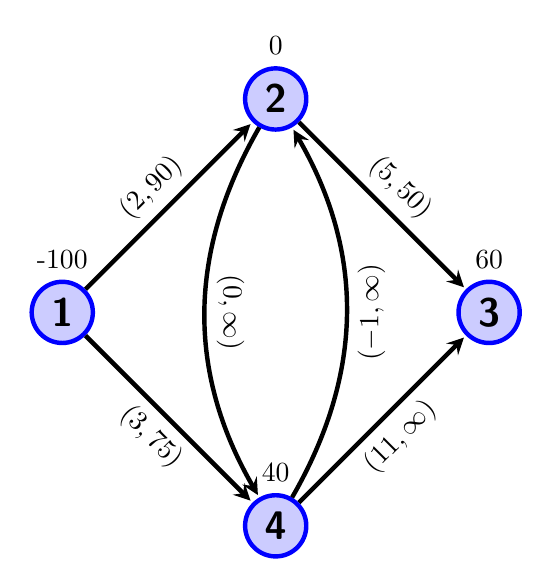
\begin{tikzpicture}[shorten >=1pt, auto, node distance=3cm, ultra thick,
  node_style/.style={circle,draw=blue,fill=blue!20!,font=\sffamily\Large\bfseries},
  edge_style/.style={draw=black, ultra thick},
  arrow_style/.style={draw=black, ultra thick,-stealth},
  every edge quotes/.append style = {anchor=north, sloped}],
                      
  \node (v1) [node_style, label=-100] {1};
  \node (v2) [node_style, label=0, above right=of v1] {2};
  \node (v3) [node_style, label=60, below right=of v2] {3};
  \node (v4) [node_style, label=40, below right=of v1] {4};
  %
  \draw [arrow_style] (v1) edge node[above,sloped]{$(2,90)$} (v2);
  \draw [arrow_style] (v1) edge node[below,sloped]{$(3,75)$} (v4);
  \draw [arrow_style,bend right] (v4) edge node[below,sloped]{$(-1,\infty)$} (v2);
  \draw [arrow_style,bend right] (v2) edge node[above,sloped]{$(0,\infty)$} (v4); 
  \draw [arrow_style] (v2) edge node[above,sloped]{$(5,50)$} (v3);    
  \draw [arrow_style] (v4) edge node[below,sloped]{$(11,\infty)$} (v3); 
      \end{tikzpicture}

\begin{enumerate}
  \item Formulate the corresponding minimum cost network flow model
  \item Classify the nodes as {\em source}, {\em sink} or {\em transshipment}
\end{enumerate}

\Answer 

In this  problem, vertex and edges are:
\begin{eqnarray*}
  V&=&\{1,2,3,4\}\\
  A&=&\{(1,2),(1,4),(2,3),(2,4),(4,2),(4,3)\}
\end{eqnarray*}

we can use the variables $x_{i,j}$ to represent the flows in the different members of set $A$. Thus, the formulation of the problem is:
\begin{equation*}
  \begin{aligned}
    \text{min} \quad&2x_{1,2}+3x_{1,4}+5x_{2,3}-x_{4,2}+11x_{4,3} \\
    \text{subject to }\quad &
    \syssubstitute{A{x_{1,2}}B{x_{1,4}}C{x_{2,3}}D{x_{2,4}}E{x_{4,3}}F{x_{4,2}}}
\systeme[ABCDEF]{
  -A-B=-100,
  A+F-C-D=0,
  C+E=60,
  B+D-F-E=40,
  A\leq 90,
  B\leq 75,
  C\leq 50} 
\end{aligned}\\
\end{equation*}
and $x_{i,j}\geq 0$.

There are 4 KKT conditions for optimal primal ($x4$) and dual ($\lambda$) variables. If $x^*$ denotes optimal values:
\begin{enumerate}
  \item Primal feasibility: all constraints must be satisfied: $g_i(x^*)-b_i$ is feasible. Applies to both equality and non-equality constraints.
  \item Gradient condition or No feasible descent: No possible improvement at the solution: 
  \[ \nabla f(x^*)-\sum_{i=1}^m \lambda_i^* \nabla g_i (x^*)=0\]
  \item Complementariety slackness: 
  \[\lambda_i^* (g_i(x^*)-b_i)=0\]
  \item Dual feasibility: $\lambda_i^*\geq 0$
\end{enumerate}

The last two conditions (3 and 4) are only required with inequality constraints and enforce a positive Lagrange multiplier when the constraint is active (=0) and a zero Lagrange multiplier when the constraint is inactive (>0). 

to solve our problem, first we will put it in its standard form:


\begin{equation*}
  \begin{aligned}
    \text{min } f(x,y)=-xy \\
    \text{subject to }\quad &
    \begin{array}{rcl}
      -x-y+100  & \geq & 0  \\
      -x-40 & \geq & 0  \\
    \end{array}
  \end{aligned}
\end{equation*}

We will go through the different conditions:

\begin{enumerate}
  \item Primal feasibility:  $g_i(x^*)-b_i$ is feasible. 
  \[-x^* -y^* +100 =0\]
  \[-x^*-40=0\]
  \item Gradient condition or No feasible descent:  
  \[ \begin{pmatrix}\pdv{f}{x}\\\pdv{f}{y}\end{pmatrix} 
  -\lambda_1 \begin{pmatrix}\pdv{g_1}{x}\\\pdv{g_1}{y}\end{pmatrix}
  -\lambda_2 \begin{pmatrix}\pdv{g_2}{x}\\\pdv{g_2}{y}\end{pmatrix} =0\]
  which, in this example, resolves into:
  \[\systeme[xy\lambda_1\lambda_2]{-y+\lambda_1+\lambda_2=0,-x-\lambda_1=0 }\]
  \item Complementariety slackness: 
  \[\lambda_1^* (-x^* -y^* +100)=0\]
  \[\lambda_2^* (-x^*-40)=0\]
  \item Dual feasibility: $\lambda_1,\lambda_2\geq 0$
\end{enumerate}

We can put the resulting 5 expressions for conditions 1 and 2 into matrix form:

\[
  \begin{pmatrix} -1 & -1 & 0&0\\ -1&0&0&0\\ 0&-1&1&1\\ -1&0&-1&0 \end{pmatrix}
  \begin{pmatrix} x\\y\\\lambda_1\\\lambda_2\end{pmatrix}=
  \begin{pmatrix} -100\\ 40\\0\\0 \end{pmatrix}
\]

  % \begin{minipage}[t]{\linewidth}
  %   \vspace{-2ex}
  %   %\includegraphics[width=\textwidth]{../figures/Afiquadrilater.pdf}
  %   \captionof{figure}{Transformacions afins d'un quadrilàter de vèrtex $(4,0)$, $(2,2)$, $(1,1)$ i $(2,-1)$.}
  %   \label{fig:trafquadril}
  % \end{minipage}



\end{ExerciseList}

\bibliography{refs}

\end{document}
